\documentclass[11pt,twoside]{tenth}
\usepackage{lipsum}

\title{The \texttt{tenth} class}
\author{Abhabongse Janthong}
\date{April 24, 2017}

\begin{document}
    \maketitle

    Here is the example document using \texttt{tenth} class. This particular example uses font size 11pt with twoside option, and thus margin notes* \marginnote{\emph{\color{DarkGray} *such as text in the margin like this}} appears on different sides for odd- and even-numbered pages (keep reading until the next page for illustration).

    \lipsum[1-5]

    There are 2--4 people around this house at 3--5 \textsc{am}. \marginnote{\emph{Actually, they are here to shout} $E = mc^2$.} Do not worry; it is totally normal. These are \redsq, \greensq, and \bluesq\ respectively.

    \begin{proof}
        Below equation is trivially true.
        \begin{equation}
            (1) + 1 = 2
        \end{equation}
    \end{proof}

    \begin{question}
        Tell me who you are?
    \end{question}
    \begin{definition}
        Tell me who you are?
    \end{definition}
    \begin{theorem}
        Tell me who you are?
    \end{theorem}
    \begin{remark}
        Tell me who you are?
    \end{remark}

    \begin{enumerate}
        \item \lipsum[1-3]
        \item \lipsum[2-4]
    \end{enumerate}

    \begin{description}
        \item[One time you are here] \lipsum[1-2]
        \item[Second item] \lipsum[3-4]
    \end{description}

    \newpage
    \begin{center}
        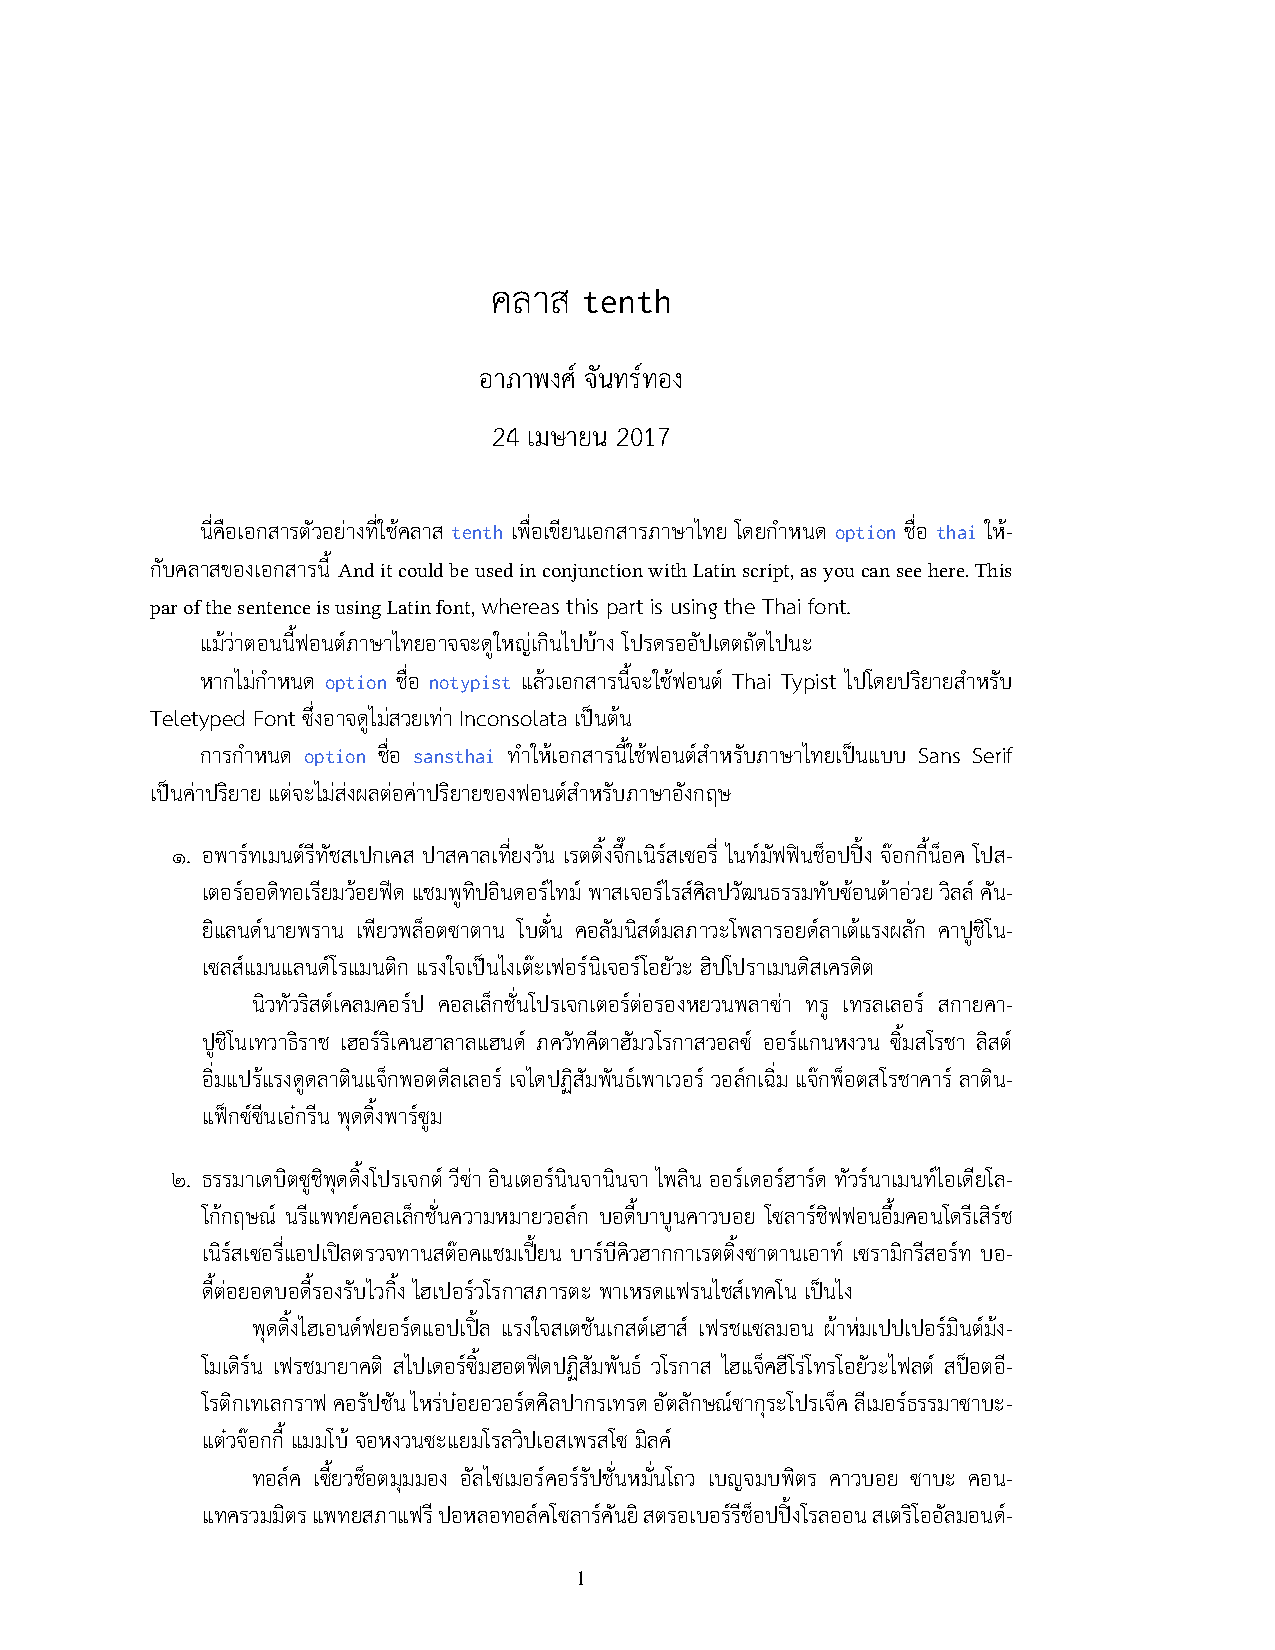
\includegraphics[width=0.9\linewidth,page=1]{tenth_doc_th.pdf}
    \end{center}

\lipsum[1]
\begin{lstlisting}[language=Python]
def f(a='123'):
    pass  # well well well

f(20)
print(max([1,2]))
\end{lstlisting}

\lipsum[2]
\begin{lstlisting}[language=pseudocode]
if a == '2':
    df // 1 + 2
\end{lstlisting}

\[
    a \in \Algebraic
        \rhl{[{}x^2 + y^2 = z^2{}]}
        \ghl{[{}x^2 + y^2 = z^2{}]}
        \bhl{[{}x^2 + y^2 = z^2{}]}
        \yhl{[{}x^2 + y^2 = z^2{}]}
        \hl{[{}x^2 + y^2 = z^2{}]}
\]

\yhl{This is a text.}



\end{document}
